 \documentclass[presentation, bigger]{beamer}
\usepackage[utf8]{inputenc}
\usepackage[T1]{fontenc}
\usepackage{fixltx2e}
\usepackage{graphicx}
\usepackage{longtable}
\usepackage{float}
\usepackage{wrapfig}
\usepackage[normalem]{ulem}
\usepackage{textcomp}
\usepackage{marvosym}
\usepackage{wasysym}
\usepackage{latexsym}
\usepackage{amssymb}
\usepackage{amstext}
\usepackage{hyperref}
\usepackage{url}
\usepackage{multimedia}
\usepackage[dutch]{babel}
\usepackage[font=scriptsize,labelfont=bf]{caption}
\setbeamertemplate{caption}[numbered]
% \usepackage{pgfpages}
% \setbeameroption{show notes on second screen=right}
\setbeamercolor*{block body example}{bg= blue!5}
\usepackage{tikz}

\tolerance=1000
\usetheme{kuleuven}
\useinnertheme{rectangles}
\graphicspath{{graphics/}}
\usepackage[style=authoryear,hyperref,backref,square,natbib,ibidtracker=false]{biblatex}
\bibliography{bibliography}

\usepackage{graphicx}
\usetheme{default}
\author{Ward Schodts, Xavier Goás Aguililla}
\date{Dinsdag 5 mei 2015}
\title{Internet of Things code deployment metrics}
\newcommand{\aheader}[2]{\action<#1-|alert@#1>{#2}}
% first argument: slide number to appear from, second argument: content of header 
\newcommand{\hiddencell}[2]{\action<#1->{#2}}
% first argument: slide number to appear from, second argument: content of cell

\DeclareBibliographyCategory{papers}


\begin{document}

\maketitle
\begin{frame}[noframenumbering]{Outline}
  \tableofcontents
  \note{3 grote luiken\\
  }
\end{frame}



\section{Inleiding}
\begin{frame}{Wireless sensor networks}

  \begin{figure}
    \fbox{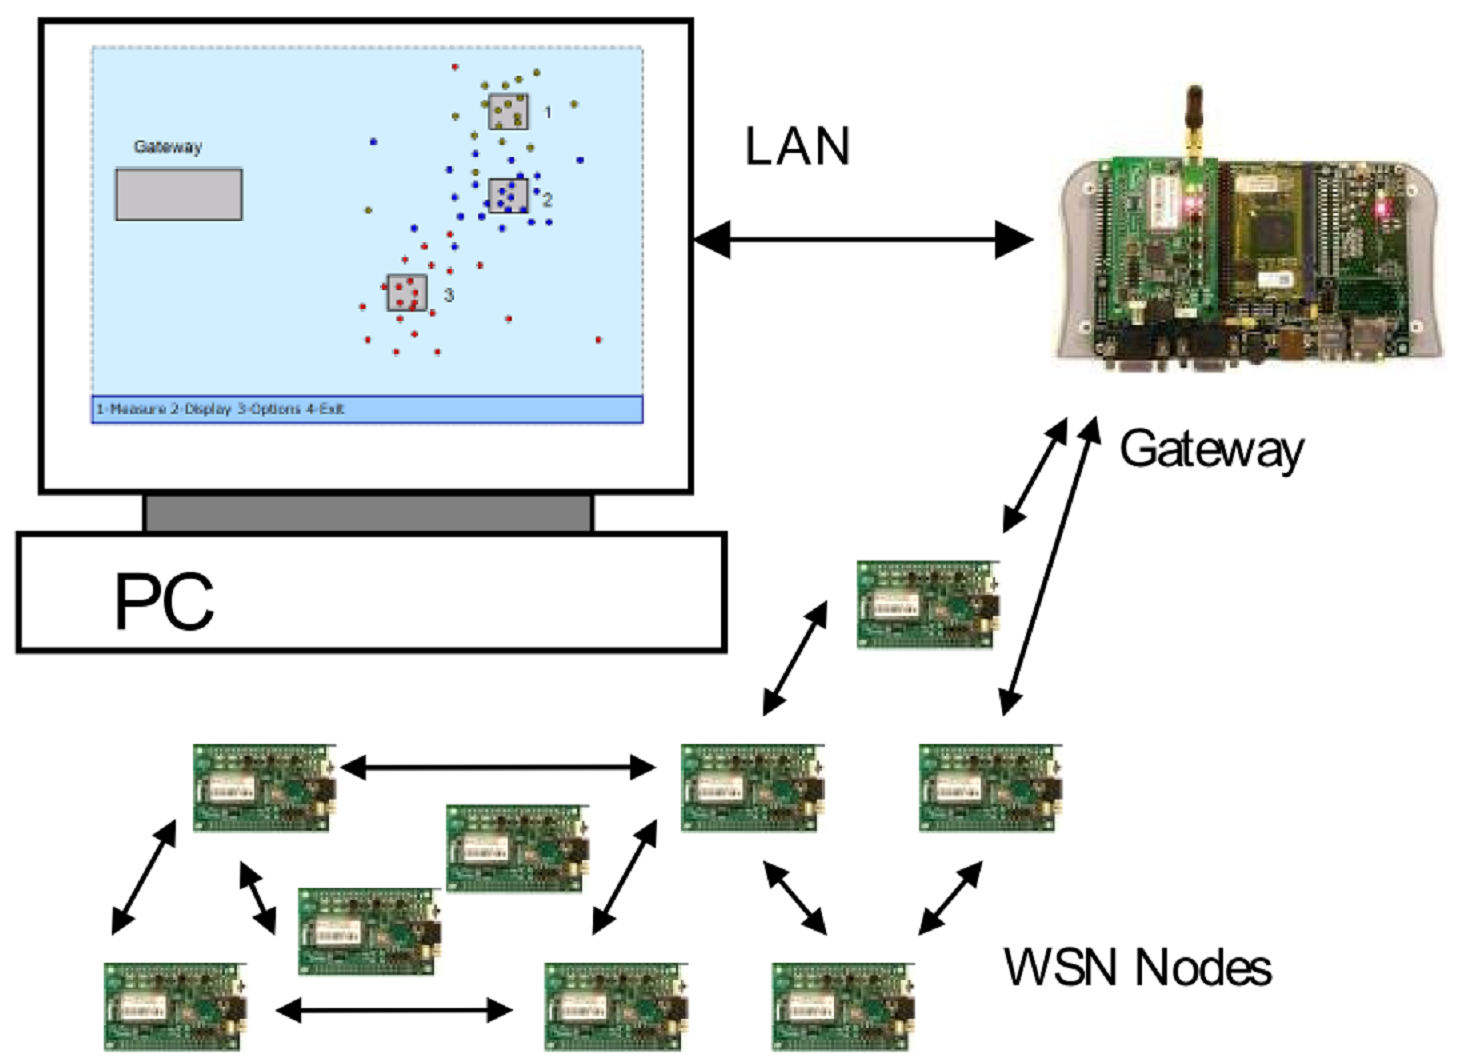
\includegraphics[width=0.82\textwidth,keepaspectration=true]{intro/overview.png}}
    \caption{Een wireless sensor network}
  \end{figure}
  \note{
    \begin{itemize}
    \item heel veel, sensoren enkele gateways
    \item netwerk bestaande uit sensoren
    \item ad-hoc netwerk technieken, geen bestaande!
    \item geen routing door 1 centrale unit
    \item communiceren via elkaar

    \end{itemize}
  }
\end{frame}

\begin{frame}{Wireless sensor networks}
  \begin{figure}
    \fbox{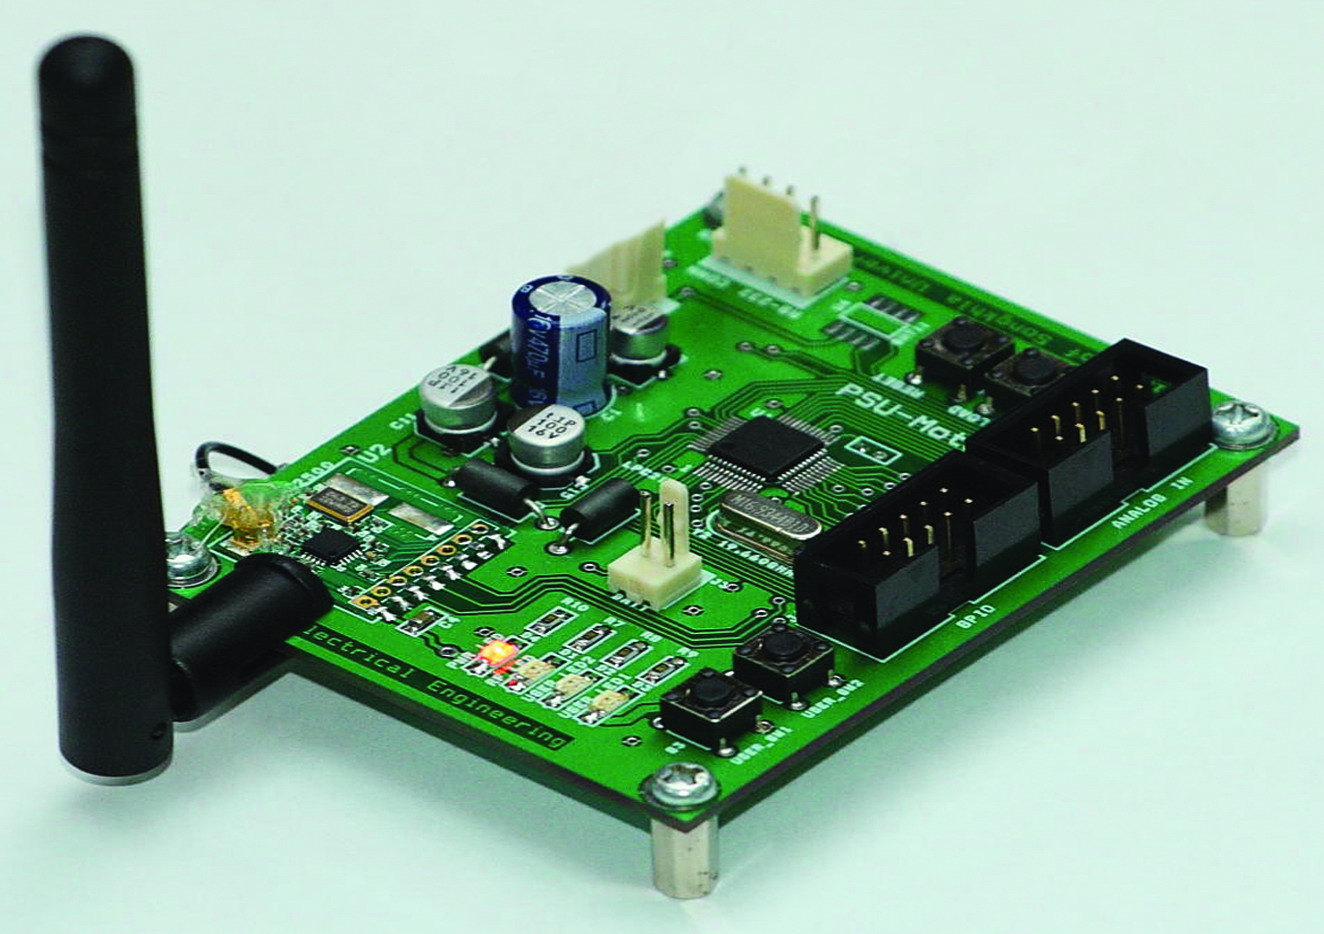
\includegraphics[height=0.78\textheight,keepaspectration=true]{intro/psumote.jpg}}
    \caption{Een PSUMote}
  \end{figure}
  \note{
    \begin{itemize}
    \item embedded device
    \item RF antenne, geen wifi, minder energie, groter bereik
    \item sensoren worden aangesloten
    \item microcontroller COMPUTEr ON A CHIP
    \end{itemize}
  }
\end{frame}

\begin{frame}{Belangrijke aspecten bij WSN-design}
  \uncover<2->{\begin{block}{energie-effici\"ent}
      tot 10 jaar meegaan op \'e\'en batterij
    \end{block}}%
  \uncover<3->{\begin{block}{dichtheid}
      tot 20 sensor nodes per $m^3$ (geen harde limiet)
    \end{block}}%
  \uncover<4->{\begin{block}{goedkoop}
      \$1 of minder voor heel grootschalige deployments
    \end{block}}%
  \uncover<5->{\begin{block}{autonoom}
      deploy and forget
    \end{block}}%
  \uncover<6->{\begin{block}{adaptief}
      makkelijke aanpasbare topologie, bestand tegen falen van motes
    \end{block}}
  \note{
    \begin{itemize}
    \item energie efficeit tot 10 jaar
    \item dichtheid, zie geneeskunde
    \item grote hoeveelheid, dus moet goedkoop, moet kapot gaan
    \item autonoom deploy and forget
    \item adaptief, topologie verandert, falende motes
    \end{itemize}}
\end{frame}



\section{Probleemstelling}

\begin{frame}{Probleemstelling}
\hiddencell{1}{	\large{Onze focus: \textbf{energie-efficiëntie}.}}
\hiddencell{2}{
\begin{exampleblock}{}
  {\textbf{Onderzoeksvraag:} is het energie-efficiënter om gegevens te verwerken op een embedded IoT toestel of op de back-end van het systeem?}
\end{exampleblock}}

\hiddencell{3}{
\begin{center}

\begin{tikzpicture}
\filldraw[blue_kuleuven] (0,0) -- (5,0) -- (2.5,-1) -- (0,0);
\node[text width=3cm] at (2.34,-0.25) {\textcolor{white}{Concretisering}};
\end{tikzpicture}
 
\end{center}
\begin{exampleblock}{}
  {\textbf{Onderzoeksopgave:} introduceer een simpele ?metric? om vlug te kunnen bepalen waar er bepaalde code moet uitgevoerd worden.}
\end{exampleblock}
}
\end{frame}

\section{Methodologie}
\begin{frame}{Methodologie}
\large{Energie berekenen voor:}
\vfill
\begin{tabular}{c c c}
      \hiddencell{2}{
\includegraphics[width=0.25\textwidth,keepaspectration=true]{storage}} & \hiddencell{3}{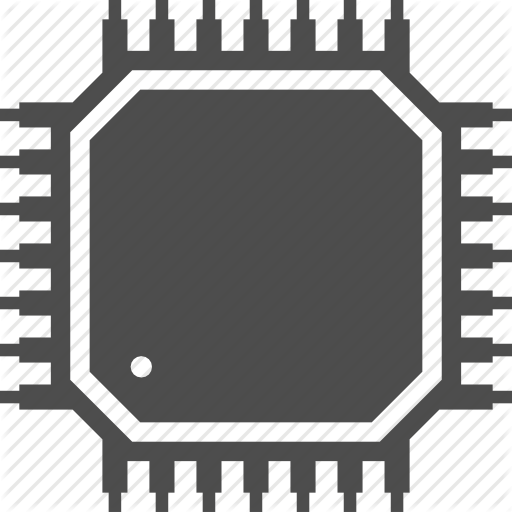
\includegraphics[width=0.25\textwidth,keepaspectration=true]{cpu}} & \hiddencell{4}{
\includegraphics[width=0.25\textwidth,keepaspectration=true]{radio}}  \\
      \hiddencell{2}{flash-opslag} & \hiddencell{3}{berekeningen} & \hiddencell{4}{netwerkoverdracht}
    \end{tabular}

\end{frame}

\section{Voorgestelde oplossing}

\begin{frame}{Voorgestelde oplossing}

\end{frame}

\section{Resultaten \& demo}
\begin{frame}{Resultaten}

\end{frame}

\begin{frame}{Demo}
\begin{center}
\Huge{Demo}
\end{center}
\end{frame}

\section{Conclusie \& verder werk}
\begin{frame}{Conclusie}
Voor of na verder werk laten komen?
\end{frame}

\begin{frame}{Verder werk}
\end{frame}

%%%%%%%%%%%%%%%%%%%%%%%%%%%%%%%%%%%%%%%%%%%%%%%%%%%%%%%%%%%%%%%
\begin{frame}[allowframebreaks]{Bibliografie}

%  \addtocategory{papers}{akyildiz2002wireless}
%  \addtocategory{papers}{mainwaring2002wireless}
%  \addtocategory{papers}{hughes2009looci}
%  \addtocategory{papers}{hughes2013energy}
  \nocite{*}
%  \textbf{Papers}
%  \printbibliography[category=papers]
%  \newpage
%  \textbf{Afbeeldingen}
%  \printbibliography[type=misc]
  \printbibliography
\end{frame}

\end{document}